% Separate manuscript edition retaining measured results and methodological limitations.
\documentclass[letterpaper,twoside]{article}
\usepackage{aistats2027}
\usepackage[hyphens]{url}
\usepackage{graphicx}
\usepackage{float}
\urlstyle{rm}
\def\UrlFont{\rm}
\usepackage[round,authoryear]{natbib}
\usepackage{booktabs}
\usepackage{amsmath}
\usepackage{amssymb}
\usepackage{amsthm}
\newtheorem{mosaictheorem}{Theorem}
\newtheorem{mosaiclemma}{Lemma}
\newtheorem{mosaicproposition}[mosaictheorem]{Proposition}
\frenchspacing

\renewcommand{\bibsection}{\subsubsection*{References}}
\bibliographystyle{apalike}
\usepackage[hidelinks]{hyperref}
\hypersetup{pdftitle={MoSAIC: Modular Self-Attentive Interacting Columns for Recurrent Memory},pdfauthor={}}

\begin{document}

\twocolumn[
\aistatstitle{MoSAIC: Modular Self-Attentive Interacting Columns\\for Recurrent Memory}

\aistatsauthor{Anonymous Author(s)}

\aistatsaddress{Anonymous Institution}

]

\begin{abstract}
Recurrent models preserve a fixed-size state, but conventionally organize it as one monolithic stream per layer. MoSAIC (Modular Self-Attentive Interacting Columns) instead factorizes state into persistent GRU columns and routes information among them with attention. We study this organization on Store--Distract--Query (SDQ) and text8 with a one-billion-token training budget. At approximately ten million parameters, L2C4 obtains $0.843 \pm 0.005$ SDQ Acc++ versus $0.544 \pm 0.074$ for GRU-L2 and $0.618 \pm 0.005$ for the strongest GRU. Acc++ is a curriculum-dependent online diagnostic. On text8, L2C4 and L3C4 obtain $1.440 \pm 0.005$ and $1.435 \pm 0.002$ validation bits per character, versus $1.483 \pm 0.006$ for the strongest GRU and $1.449 \pm 0.012$ for a finite-context Transformer. An additional one-million-parameter series reproduces the improvement over GRU, but a local Mamba baseline performs better. These internal comparisons support a task-dependent benefit of modular recurrent organization, without isolating it from state capacity or establishing general superiority.
\end{abstract}

\section{Introduction}

Recurrent networks compress sequence history into a fixed-size state and update it incrementally. A conventional GRU \citep{cho2014gru} or LSTM \citep{hochreiter1997lstm}, however, represents each layer as a single hidden-state stream. Width or depth adds capacity but leaves the organization and exchange of information within that state implicit.

How should a fixed recurrent parameter budget be organized into persistent modules with learned communication, and how do depth and column count affect outcomes? We distinguish memory organization, state capacity, and routing computation: components maintain local state while content-dependent routing moves information among them. A parameter-matched topology sweep can reveal non-monotonic relationships with state volume, while causal attribution requires additional state-matched controls.

We introduce \emph{MoSAIC (Modular Self-Attentive Interacting Columns)}, which distributes each layer across independently parameterized GRU columns. Each column queries a small message bank before its recurrent update. The bottom layer reads the current input and delayed top-layer states; higher layers read the newly updated states below. All columns update, and the top layer persists to the next timestep.

``Self-Attentive'' denotes attention over $C+1$ messages at the bottom layer and $C$ above, where $C$ is the column count. Bank size is independent of token history; every column updates synchronously.

We evaluate the original ten-million-parameter models on SDQ and text8, and add a one-million-parameter text8 series with recorded seeds, modern recurrent baselines, RIMs/BRIMs, and routing controls. Both series use a one-billion-token training budget. L2C4 is the compact two-layer reference, and L3C4 has the best observed MoSAIC mean. Short component ablations and exploratory LRU, associative-recall, and reinforcement-learning experiments test the boundaries of this result.

Our contributions are:
\begin{itemize}
    \item \textbf{Architecture:} a layered grid of persistent recurrent columns with attention-mediated inter-column communication.
    \item \textbf{Conditional analysis:} a local Gaussian model characterizes source fusion, optimal prediction through a compressed readout, and the limits of column-count arguments.
    \item \textbf{Topology result:} among the evaluated two-layer shapes at approximately fixed parameter scale, wider grids have more state and a higher SDQ diagnostic, but worse text8 BPC. Column count and within-column width change jointly.
    \item \textbf{Replication and boundaries:} improvements over GRU recur at two parameter scales; the smaller-scale series adds modular and modern baselines, sparse-routing controls, and component pilots. Mamba's stronger text8 result and weak recall/RL transfer delimit the claim.
\end{itemize}

\section{Related Work}

\paragraph{Modular recurrence and communication.}
Recurrent Independent Mechanisms (RIMs) \citep{goyal2019rims} maintain separate recurrent modules, sparsely activate a subset for each input, and allow active modules to communicate through attention. BRIMs \citep{mittal2020brims} add hierarchical bottom-up and top-down communication, while shared-workspace models \citep{goyal2021workspace} impose a communication bottleneck. Relational Memory Core \citep{santoro2018relational} updates interacting memory slots through attention. Object files and schemata \citep{goyal2021factorizing} factorize persistent object states and shared update rules. Spatially Structured Recurrent Modules \citep{rahaman2021spatial} learn interactions informed by spatial structure. MoSAIC shares bottom-up and delayed top-down information flow with BRIMs; its design combines independent GRUs, synchronous updates of every column, and a single-column readout. Our text8 experiments compare local RIMs/BRIMs implementations under a common recipe.

\paragraph{Grid and multidimensional recurrence.}
Multi-Dimensional RNNs \citep{graves2007mdrnn} propagate information recurrently along multiple axes of structured data. Grid LSTM \citep{kalchbrenner2015gridlstm} arranges LSTM blocks in a multidimensional grid whose dimensions exchange hidden and memory vectors through fixed connections. MoSAIC uses a grid as an organization of modules rather than as an additional axis of the input. All columns share one temporal axis, retain separate recurrent states, and communicate through content-dependent routing rather than edges fixed by input geometry.

\paragraph{Modern recurrent and attention models.}
Recent architectures redesign recurrent updates or memory representations: LRUs \citep{orvieto2023lru} use stabilized linear recurrences, HGRN2 \citep{qin2024hgrn2} expands gated linear state, Mamba \citep{gu2023mamba} selects state-space dynamics from inputs, Mamba-2 \citep{dao2024mamba2} relates state-space models to structured attention, DeltaNet \citep{yang2024deltanet} uses delta-rule matrix state, and xLSTM \citep{beck2024xlstm} includes scalar and matrix memory. Transformers \citep{vaswani2017attention} and Transformer-XL \citep{dai2019transformerxl} retain token representations for attention. Our new equal-token series compares local implementations of Mamba, HGRN2, DeltaNet, and mLSTM. The Mamba reference is a sequential selective-SSM implementation, not Mamba-2. Older reduced-token runs remain separate implementation context (Appendix~\ref{app:reduced}).

\paragraph{Routing and associative memory.}
Sparse mixture-of-experts layers \citep{shazeer2017moe,fedus2021switch} select subsets of parameterized experts for individual inputs. MoSAIC routes messages among persistent columns that all update. Neural Turing Machines \citep{graves2014ntm} learn attention-based access to external memory. Recall benchmarks \citep{arora2023zoology} and induction-head analyses \citep{olsson2022induction} motivate associative retrieval tests. We distinguish the curriculum-dependent SDQ diagnostic from an additional multi-query associative recall (MQAR) pilot; neither establishes in-context learning in natural language.

\begin{figure*}[t]
\centering
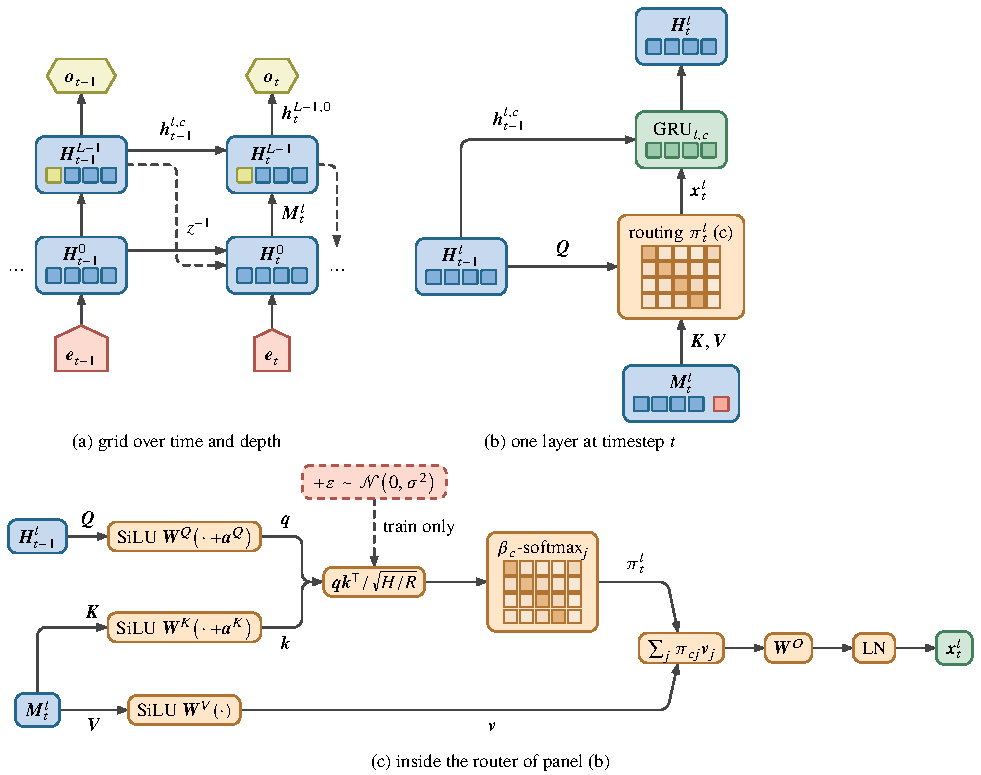
\includegraphics[width=\textwidth]{fig_architecture.pdf}
\caption{MoSAIC mechanism. At timestep $t$, each persistent column state queries a layer-specific message bank. The first layer reads the current input together with the previous top-layer column states; later layers read the newly updated states below them. The routed message is the input to an independent recurrent update. All top-layer column states are carried to timestep $t+1$.}
\label{fig:architecture}
\end{figure*}

\section{Method}\label{sec:method}

\subsection{Persistent Columns and Layered Topology}

Let $\mathbf{e}_t \in \mathbb{R}^{B \times H}$ be an embedded input for a batch of size $B$. A conventional $L$-layer GRU maintains $\mathbf{S}_t \in \mathbb{R}^{L \times B \times H}$. MoSAIC instead maintains
\begin{equation}
    \mathbf{H}_t \in \mathbb{R}^{L \times C \times B \times H},
\end{equation}
where $\mathbf{h}_t^{l,c}$ denotes column $c$ at layer $l$. Each layer--column pair has independent GRU parameters. Columns in a layer are evaluated together for efficiency, but do not share recurrent weights.

The message bank for the first layer contains the delayed top layer and the current external inputs:
\begin{equation}
    \mathbf{M}_t^0 =
    [\mathbf{H}_{t-1}^{L-1}; \mathbf{e}_t]
    \in \mathbb{R}^{(C+1) \times B \times H}.
\end{equation}
Each experiment uses one input stream. At subsequent layers,
\begin{equation}
    \mathbf{M}_t^l = \mathbf{H}_t^{l-1}, \qquad l > 0.
\end{equation}
Information therefore moves bottom-up within a timestep, while the complete top layer provides a delayed feedback path across timesteps. Figure~\ref{fig:architecture} summarizes this computation.

\subsection{Attention-Mediated Routing}

Layers and columns are indexed from zero. At layer $l$, the previous states of its $C$ columns form the queries. Learnable identities $\mathbf{a}_c^{Q,l},\mathbf{a}_j^{K,l}\in\mathbb{R}^{H}$ distinguish query columns and message sources. With $R$ heads, each head has dimension $d=H/R$ and projection matrices $\mathbf{W}_r^{Q,l},\mathbf{W}_r^{K,l},\mathbf{W}_r^{V,l}\in\mathbb{R}^{d\times H}$ and biases in $\mathbb{R}^{d}$. The output projection has $\mathbf{W}^{O,l}\in\mathbb{R}^{H\times H}$ and $\mathbf{b}^{O,l}\in\mathbb{R}^{H}$. For head $r$,
\begin{align}
\mathbf{q}_{t,c,r}^l &=
    \operatorname{SiLU}\!\left(
    \mathbf{W}_r^{Q,l}(\mathbf{h}_{t-1}^{l,c}+\mathbf{a}_c^{Q,l})+\mathbf{b}_r^{Q,l}
    \right), \\
\mathbf{k}_{t,j,r}^l &=
    \operatorname{SiLU}\!\left(
    \mathbf{W}_r^{K,l}(\mathbf{m}_{t,j}^l+\mathbf{a}_j^{K,l})+\mathbf{b}_r^{K,l}
    \right), \\
\mathbf{v}_{t,j,r}^l &=
    \operatorname{SiLU}\!\left(
    \mathbf{W}_r^{V,l}\mathbf{m}_{t,j}^l+\mathbf{b}_r^{V,l}
    \right).
\end{align}
Each query column has a learned positive inverse temperature $\beta_c^l=\operatorname{softplus}(\rho_c^l)$. The routing probabilities are
\begin{equation}
\pi_{t,c,j,r}^l =
\operatorname{softmax}_j\!\left[
\beta_c^l\left(
\frac{\mathbf{q}_{t,c,r}^l \cdot \mathbf{k}_{t,j,r}^l}{\sqrt{H/R}}
+ \epsilon_{t,c,j,r}^l
\right)\right],
\end{equation}
where $R$ is the number of heads. The perturbation $\epsilon\sim\mathcal{N}(0,\sigma_\epsilon^2)$ is independent during training and zero at evaluation. Noise is added before temperature scaling, so its effective logit standard deviation is $\beta_c^l\sigma_\epsilon$. SiLU \citep{elfwing2018silu} is applied to all three projections. Query and key identities distinguish participants; values carry projected content without an identity offset. These projection choices have not been individually ablated. Concatenated head outputs are linearly projected and layer-normalized:
\begin{equation}
\begin{aligned}
\mathbf{z}_{t,c,r}^l
    &= \sum_j \pi_{t,c,j,r}^l\mathbf{v}_{t,j,r}^l,\\
\mathbf{u}_{t,c}^l
    &= \mathbf{W}^{O,l}[\mathbf{z}_{t,c,1}^l;\ldots;\mathbf{z}_{t,c,R}^l]
       +\mathbf{b}^{O,l},\\
\mathbf{x}_{t,c}^l
    &= \operatorname{LN}(\mathbf{u}_{t,c}^l).
\end{aligned}
\end{equation}
Routing determines the input to each recurrent cell; it does not replace or post-process its persistent state.

\subsection{Recurrent Update and Readout}

Every column performs an ordinary independent GRU update,
\begin{equation}
\mathbf{h}_t^{l,c} =
\operatorname{GRU}_{l,c}
(\mathbf{x}_{t,c}^l,\mathbf{h}_{t-1}^{l,c}).
\end{equation}
The prediction head reads column 0 of the top layer. This intentional readout bottleneck requires useful information held in peripheral columns to be compressed and retrieved through one column. All top-layer columns persist and participate in the next bottom-layer message bank.

The full MoSAIC configuration uses three training-only routing terms: Gaussian logit noise, a communication cost favoring diagonal routes, and an entropy bonus favoring higher routing entropy. Let $S_l$ be the number of messages at layer $l$. With zero-based column index $c$, the route cost $d_{c,j}^l$ is zero for the same-column recurrent message, one for another recurrent message, and $2c$ for the external input at the bottom layer. The communication loss is the mean expected route cost,
\begin{equation}
\mathcal{L}_{\mathrm{comm}}
= \mathbb{E}_{t,l,c,r}\!\left[
\sum_{j=0}^{S_l-1}\pi_{t,c,j,r}^l d_{c,j}^l
\right].
\end{equation}
Routing entropy is normalized by the log of the number of available messages,
\begin{equation}
\overline{\mathcal{H}}(\pi)
= \mathbb{E}_{t,l,c,r}\!\left[
\frac{-\sum_{j=0}^{S_l-1}\pi_{t,c,j,r}^l
\log \pi_{t,c,j,r}^l}{\log S_l}
\right].
\end{equation}
For task loss $\mathcal{L}_{\mathrm{task}}$,
\begin{equation}
\mathcal{L} =
\mathcal{L}_{\mathrm{task}}
+ \lambda_{\mathrm{comm}}\mathcal{L}_{\mathrm{comm}}
- \lambda_{\mathrm{ent}}\overline{\mathcal{H}}(\pi).
\end{equation}
Full MoSAIC configurations use four routing heads. For text8, $(\lambda_{\mathrm{comm}},\lambda_{\mathrm{ent}},\sigma_\epsilon)=(0.05,0.005,0.05)$; for SDQ, the settings are $(0.02,0.002,0.02)$. Section~\ref{sec:ablation} disables these terms individually and together in short text8 pilots; their contribution to the full-budget SDQ result remains untested. The LRU extensions use different routing and no auxiliary losses, so they are not isolated GRU-to-LRU cell substitutions.

\subsection{Fixed-State and Resource Accounting}

Attention is applied over $C+1$ messages in the bottom layer and $C$ messages above it. For fixed $L$, $C$, and $H$, the carried recurrent state and per-token routing geometry are independent of processed sequence length.

Ignoring embeddings and biases, the independent GRUs contribute approximately $6LCH^2$ parameters and routing projections approximately $4LH^2$. Persistent state contains $LCH$ scalars per example, compared with $LH$ for a stacked GRU. Parameter matching consequently does not match activation state or computation. Projection and GRU work is $O(L(C+1)H^2)$ per example and token, while attention products require $O([C(C+1)+(L-1)C^2]H)$ work. Routing weights occupy $O(R[C(C+1)+(L-1)C^2])$ transient scalars per example, in addition to projections and GRU intermediates. Table~\ref{tab:topology} gives carried-state sizes and float32 storage; these are not peak training-memory measurements.

\subsection{A Local Bayesian Model of Routing}\label{sec:bayesian}

We analyze information access at a fixed timestep, receiver, and scalar projected-message coordinate. This surrogate uses standard Gaussian fusion \citep{murphy2007gaussian}; it is not a distributional claim about learned GRU states.

\paragraph{Assumption G.}
Let $A$ be a finite source set and $Z\sim\mathcal{N}(m_0,\tau_0^{-1})$, with $\tau_0>0$. For each $i\in A$, let $M_i=Z+\varepsilon_i$, where the noises are mutually independent, independent of $Z$, and $\varepsilon_i\sim\mathcal{N}(0,\tau_i^{-1})$ with fixed known $\tau_i>0$. Source subsets are fixed before observing messages. Any recurrent history treated as context must leave this conditional model valid.

For nonempty $S\subseteq A$, write $M_S=(M_i)_{i\in S}$ and define
\begin{equation}\label{eq:bayesian-definitions}
\begin{aligned}
T_S &= \sum_{i\in S}\tau_i,\qquad \bar T_S=\tau_0+T_S,\\
\mu_S &= \frac{\sum_{i\in S}\tau_i M_i}{T_S},\qquad
\bar\mu_S=\frac{\tau_0m_0+T_S\mu_S}{\bar T_S}.
\end{aligned}
\end{equation}

\begin{mosaictheorem}[Posterior fusion]\label{thm:posterior-fusion}
Under Assumption G, $Z\mid M_S\sim\mathcal{N}(\bar\mu_S,\bar T_S^{-1})$. In the flat-prior limit $\tau_0\downarrow0$, the normalized likelihood has mean $\mu_S$ and variance $T_S^{-1}$.
\end{mosaictheorem}

Appendix~\ref{app:bayesian} proves this result and four further theorems. Fusion uniquely minimizes a precision-weighted quadratic (Theorem~\ref{thm:fusion-optimality}). Retaining an additional independent source strictly lowers posterior variance (Theorem~\ref{thm:retained-route}) and optimal squared-error risk (Theorem~\ref{thm:bayes-risk}), holding existing precisions fixed. A compressed readout $Y=g(M_S)$ has optimal conditional risk
\begin{equation}\label{eq:bayesian-bottleneck-main}
\bar T_S^{-1}+\operatorname{Var}(\bar\mu_S\mid Y)
\geq \bar T_S^{-1},
\end{equation}
with equality exactly when $Y$ preserves the posterior mean (Theorem~\ref{thm:bottleneck}). Thus a single-column readout can preserve all information needed for optimal squared-error prediction; its dimension alone does not determine information loss.

The flat-prior weights satisfy $\tau_i/T_S=\operatorname{softmax}_{i\in S}(\log\tau_i)$, giving an algebraic correspondence to attention. MoSAIC's learned logits are not calibrated precisions, and top-$k$ selection consults all source scores. These theorems therefore describe fixed information access, not the implemented adaptive router. Changing column count can change both messages and precisions (Proposition~\ref{prop:column-count}); no monotonic quality guarantee follows. Gaussian squared-error risk is also distinct from token cross-entropy, so the analysis gives no BPC guarantee.


\section{Experiments}\label{sec:experiments}

\subsection{Protocols and Uncertainty}

The historical cohort compares approximately 10M-parameter models on SDQ and text8; the new cohort uses approximately 1M-parameter text8 models with recorded seeds. Single-seed pilots investigate routing, LRU cells, recall, and RL. Quality comparisons use validation or the identified online diagnostic; matching training budgets does not match compute or state.

We retain the original historical cohort and report the main comparisons with a 1B-token training budget. Text8 results use the final validation evaluation; SDQ results average the final five diagnostic measurements per launch. We report mean $\pm$ sample standard deviation across launches, with denominator $n-1$. Historical seeds were not recorded; new main runs have recorded seeds, specified in Appendix~\ref{app:midprotocol}. There are no significance tests, and one-seed pilots have no uncertainty estimate. Appendix~\ref{app:uncertainty} explains the limits of this reporting.

% Generated offline by inference/aistats_revision_evidence.py.
\begin{table*}[t]
\centering
\caption{Historical $\sim$10M models, reaggregated at common logged budgets. Text8: 960,036,864 tokens; Transformer BPC is linearly interpolated between bracketing logs, recurrent rows are exact. SDQ: per-launch mean over the same five logs at 950.04--970.04M tokens. Values are mean $\pm$ sample SD; SDQ has three launches per row. Params are for text8. $\dagger$: two text8 launches. Acc++ is an online curriculum diagnostic.}
\label{tab:historical}
\begin{tabular}{lrrrr}
\toprule
Model & Params & Text8 $n$ & Val. BPC $\downarrow$ & SDQ Acc++ $\uparrow$ \\
\midrule
GRU-L1 & 10.16M & 3 & $1.5641\pm0.0027$ & $0.6159\pm0.0040$ \\
GRU-L2 & 10.04M & 3 & $1.5005\pm0.0121$ & $0.5409\pm0.0735$ \\
GRU-L3 & 10.23M & 3 & $1.4839\pm0.0067$ & $0.3177\pm0.0850$ \\
MoSAIC-L1C8 & 10.11M & 3 & $1.4671\pm0.0030$ & $0.7009\pm0.0186$ \\
MoSAIC-L2C4 & 10.11M & 3 & $1.4389\pm0.0033$ & $0.8389\pm0.0062$ \\
MoSAIC-L2C8 & 10.17M & 3 & $1.4401\pm0.0010$ & $0.8641\pm0.0129$ \\
MoSAIC-L2C16$^{\dagger}$ & 10.09M & 2 & $1.4510\pm0.0014$ & $0.8830\pm0.0116$ \\
MoSAIC-L3C4 & 9.99M & 3 & $1.4349\pm0.0008$ & $0.9137\pm0.0123$ \\
Transformer-256 & 10.07M & 3 & $1.4522\pm0.0088$ & --- \\
Transformer-64 & 10.07M & 3 & $1.4826\pm0.0056$ & --- \\
\bottomrule
\end{tabular}
\end{table*}


\subsection{Historical Memory and Language Results}

\paragraph{SDQ.}
Store--Distract--Query is an online associative-storage task with overwriting, distractors, and key-dependent counters. Its evolving curriculum increases episode length and decreases store/query frequency. We train with 512 streams, BPTT length 32, RMSprop, and gradient clipping at norm 1. Appendix~\ref{app:sdq} gives the generator and target exactly. Acc++ is accuracy on valid queries with a store--query gap strictly greater than the current batch's mean valid gap. This is a changing subset of training-generator queries, not fixed-gap held-out accuracy.

MoSAIC-L2C4 reaches $0.8433\pm0.0055$, versus $0.5444\pm0.0743$ for GRU-L2 and $0.6177\pm0.0052$ for the strongest GRU, L1. L3C4 has the highest observed mean, $0.9204\pm0.0128$. Every evaluated MoSAIC shape has a higher central diagnostic than every GRU depth. Figure~\ref{fig:learning}(b) shows the trajectories; the changing curriculum limits interpretation as a fixed retrieval benchmark.

\paragraph{Text8.}
Text8 \citep{mahoney2011text8} contains 100M normalized English characters and a 27-character alphabet. Historical runs use the first 90M characters for training and the last 10M for validation, which was also used for manual configuration choices. Their BPC values are internal validation comparisons, not published text8 test results. Recurrent models use 512 contiguous streams, BPTT length 64, RMSprop, and the reset/learning-rate schedules in Appendix~\ref{app:protocol}. Evaluation disables random resets. BPC is cross-entropy in nats divided by $\log 2$.

L2C4 obtains $1.4397\pm0.0050$, versus $1.5004\pm0.0119$ for GRU-L2. L3C4 reaches $1.4345\pm0.0017$, versus $1.4830\pm0.0061$ for the strongest GRU, L3. The cache-256 Transformer reaches $1.4492\pm0.0120$. It shares the token batch, optimizer, and training target, but uses parallel segment processing and a rolling key/value cache. Its four layers have width 560, four heads, feed-forward width 1120, RMSNorm \citep{zhang2019rmsnorm}, and RoPE \citep{su2021roformer}; cache lengths 256 and 64 are separate configurations. Figure~\ref{fig:learning}(a) shows that the GRU--MoSAIC separation is visible during training.

\begin{figure*}[t]
\centering
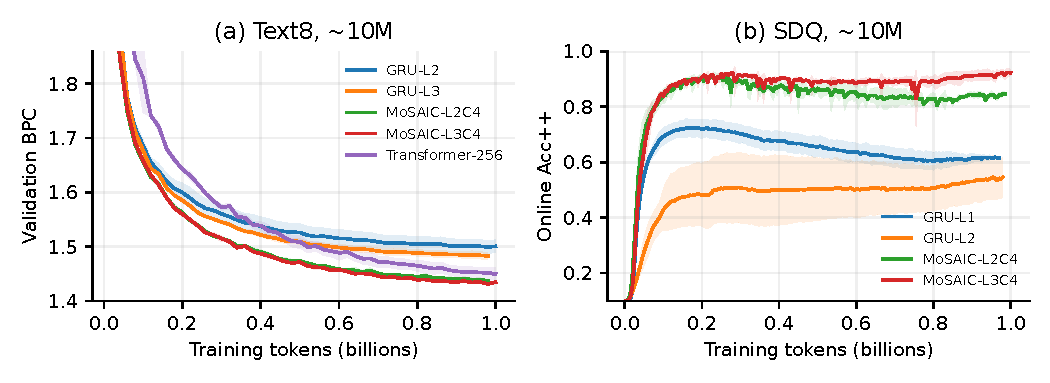
\includegraphics[width=\textwidth]{fig_aistats_historical_curves.pdf}
\caption{Historical $\sim$10M learning curves. Means and sample-SD bands across three launches per configuration with a 1B-token training budget. SDQ is an online curriculum diagnostic; historical text8 validation was consulted during configuration selection. Shading is descriptive, not a significance test.}
\label{fig:learning}
\end{figure*}

\subsection{Modern and Modular References at Smaller Scale}\label{sec:mid}

The new series uses the contiguous 90M/5M/5M train/validation/test split. It retains 512 streams, 64-step BPTT, the common optimizer/reset recipe, and a 1B-token training budget. Models include embeddings and heads and range from 0.973M to 1.069M parameters (Table~\ref{tab:mid}); matching is approximate, with state and compute separate. We evaluate the 5M validation segment with resets disabled; no test values were consulted to select architectures or construct these comparisons. A final test split is configured and some runs have logged test metrics, but we report validation throughout. The historical 10M validation segment includes this test segment, so the new split does not retroactively make it untouched by earlier development.

% Generated offline by inference/aistats_revision_evidence.py.
\begin{table}[t]
\centering
\caption{Text8 $\sim$1M series: mean $\pm$ sample SD of validation BPC. Upper panel: exactly 980,037,632 logged tokens. Lower panel uses separate horizons: $\dagger$ 960,036,864; $\ddagger$ 982,646,784, without interpolation. Seeds 42/1337, adding 31337 for $n=3$. Split 90M/5M/5M. Local baselines share the training recipe; state and compute are unmatched.}
\label{tab:mid}
\begin{tabular}{lrrr}
\toprule
Model & Params & $n$ & BPC $\downarrow$ \\
\midrule
Mamba & 1.003M & 2 & $1.5651\pm0.0012$ \\
MoSAIC L3C4 & 1.069M & 3 & $1.5916\pm0.0012$ \\
MoSAIC L2C4 & 1.050M & 3 & $1.5966\pm0.0050$ \\
MoSAIC L2C8 & 0.973M & 2 & $1.6082\pm0.0019$ \\
MoSAIC L1C8 & 1.034M & 2 & $1.6369\pm0.0016$ \\
GRU L1 & 1.004M & 2 & $1.6807\pm0.0003$ \\
GRU L2 & 1.014M & 3 & $1.6368\pm0.0018$ \\
GRU L3 & 0.986M & 2 & $1.6205\pm0.0076$ \\
Grid-LRU L1C8 & 1.004M & 2 & $1.7473\pm0.0005$ \\
Grid-LRU L2C8 & 1.060M & 2 & $1.7156\pm0.0047$ \\
Grid-LRU L3C4 & 1.063M & 3 & $1.6690\pm0.0052$ \\
HGRN2 & 0.996M & 2 & $1.6695\pm0.0005$ \\
mLSTM & 0.996M & 2 & $1.7163\pm0.0039$ \\
DeltaNet & 1.004M & 2 & $1.7849\pm0.0005$ \\
RIMs & 0.995M & 2 & $1.8744\pm0.0977$ \\
BRIMs & 1.000M & 2 & $1.8968\pm0.0318$ \\
\midrule
\multicolumn{4}{l}{Separate logged horizons:} \\
Grid-LRU L2C4$^{\dagger}$ & 1.049M & 3 & $1.6750\pm0.0032$ \\
Transformer-256$^{\ddagger}$ & 1.002M & 2 & $1.6396\pm0.0098$ \\
\bottomrule
\end{tabular}
\end{table}


MoSAIC-L2C4 achieves $1.5960\pm0.0058$ BPC versus $1.6359\pm0.0007$ for GRU-L2; L3C4 reaches $1.5918\pm0.0009$, versus $1.6205\pm0.0080$ for the strongest GRU, L3. The improvement therefore recurs at a smaller scale with recorded seeds. Local RIMs and BRIMs references obtain $1.8741\pm0.0965$ and $1.8853\pm0.0179$. Each uses six LSTM modules, three active per token; BRIMs adds delayed top-down communication. They address the absence of direct modular references, but are compact reimplementations under our shared recipe, without architecture-specific tuning or a claim to reproduce their best published results.

Mamba is stronger than MoSAIC in this series, at $1.5657\pm0.0010$ BPC. HGRN2, DeltaNet, and mLSTM now have two runs with the same training budget, replacing reduced-token comparisons at this scale. This is an internal comparison of local sequential implementations, not a ranking of optimized model families. The new cache-256 Transformer has $1.6396\pm0.0098$ BPC across two seeds in Table~\ref{tab:mid}.

The simplified Grid-LRU reference replaces GRU cells, projected content attention, and auxiliary terms with complex diagonal linear recurrence and learned static mixing, retaining column-0 readout and normalized top-layer feedback (Appendix~\ref{app:lru}). Thus it is a lighter architectural alternative, not a cell-only ablation. L2C4 Grid-LRU gives $1.6720\pm0.0006$ versus $1.5960\pm0.0058$ for MoSAIC-L2C4 ($n=3$ each). L3C4 Grid-LRU has $1.6699\pm0.0042$. Simpler updates do not preserve the text8 improvement; resource benefits require measurement.

\subsection{Routing Sparsity and Component Pilots}\label{sec:ablation}

\paragraph{Sparse message selection.}
Holding MoSAIC-L2C4 widths and routing terms fixed, seed-42 top-$k$ attention retains only the $k$ highest-scoring sources per query/head. Dense routing gives 1.5921 BPC, top-2 gives 1.6353, and top-1 gives 1.8869. Restricting source access therefore hurts this text8 configuration, most strongly at top-1. All column cells still update: source sparsity is distinct from RIMs' selective module updates and does not establish an execution speedup.

% Generated offline by inference/aistats_revision_evidence.py.
\begin{table}[t]
\centering
\caption{MoSAIC-L2C4 regularizer pilot, seed 42: validation BPC at 50,331,648 tokens. Same widths, optimizer and 524,288-token validation cap; $\Delta$ is relative to the full model. One launch per condition; no variability estimate.}
\label{tab:ablation}
\begin{tabular}{lrr}
\toprule
Condition & BPC $\downarrow$ & $\Delta$ \\
\midrule
Full & 1.9260 & $+0.0000$ \\
All three off & 1.9282 & $+0.0022$ \\
No logit noise & 1.9243 & $-0.0016$ \\
No communication cost & 1.9220 & $-0.0040$ \\
No entropy bonus & 1.9224 & $-0.0036$ \\
\bottomrule
\end{tabular}
\end{table}


\paragraph{Training terms.}
Table~\ref{tab:ablation} gives the first component test. Removing noise, communication cost, entropy bonus, or all three changes BPC by at most 0.0041 in this short pilot, with signs changing across earlier points. Removing the communication term nevertheless raises its logged expected route cost from about 0.896 to 1.045 in the routing diagnostic, while normalized entropy stays near 0.96--0.97. The term changes routing without a resolved quality benefit in this pilot. The evaluation is near the end of the reset warmup, uses one seed and a capped validation prefix, and omits full-budget SDQ. Full-budget and repeated-seed ablations are still required to assess their quality contribution.

\paragraph{Longer BPTT and LRU mechanisms.}
Length-512 pilots keep 32,768 tokens/update by reducing training streams from 512 to 64. These short pilots do not improve Grid-LRU, and GRU/MoSAIC are about 0.02 BPC worse; this does not isolate long-context capacity from trajectory diversity or training schedule (Appendix~\ref{app:rollout}). Five LRU memory/reading modifications and seven sparse-routing variants are reported with their own controls in Appendix~\ref{app:lru}. Two hub reads improve text8 by 0.0185 BPC on one seed, but this gain does not transfer to our recall/RL pilots.

% Generated offline by inference/aistats_resource_accounting.py.
\begin{table*}[t]
\centering
\caption{Historical log-derived costs for the H100 subset of the main references with a 1B-token training budget. Elapsed loop time and effective rate are per-launch means $\pm$ sample standard deviations. $\dagger$: one launch, with no variability estimate. This hardware subset has fewer launches than the quality tables; workload contention was not controlled. Time includes training-loop overhead and is not exclusive accelerator usage.}
\label{tab:resources}
\begin{tabular}{llrrr}
\toprule
Task & Model & $n$ & Loop time (h) & Rate (k tokens/s) \\
\midrule
SDQ & MoSAIC-L2C4$\dagger$ & 1 & $1.327$ & $209.3$ \\
SDQ & MoSAIC-L3C4 & 3 & $1.946\pm0.311$ & $145.4\pm25.1$ \\
SDQ & GRU-L2$\dagger$ & 1 & $0.984$ & $282.2$ \\
text8 & MoSAIC-L2C4 & 2 & $1.627\pm0.236$ & $172.5\pm25.1$ \\
text8 & MoSAIC-L3C4 & 3 & $2.264\pm0.033$ & $122.7\pm1.8$ \\
text8 & GRU-L2 & 2 & $1.097\pm0.016$ & $253.1\pm3.6$ \\
text8 & Transformer-256$\dagger$ & 1 & $0.571$ & $486.1$ \\
\bottomrule
\end{tabular}
\end{table*}


\subsection{Additional Recall and RL Probes}\label{sec:transfer}

On MQAR \citep{arora2023zoology}, the dynamic-hub LRU control answers 2.70\% of validation queries: 24.825\% with four stored pairs, falling to 0.142\% with 64 pairs. All six variants have zero sequence-level exact match; query-conditioned read stays near chance. Several runs have large gradient spikes. Appendix~\ref{app:mqar} details the independent validation generator and query-weighted aggregation. Strong-baseline comparisons are missing.

Ten single-seed POPGym \citep{morad2023popgym} pilots do not show a Grid advantage over plain LRU. RepeatPreviousHard late mean return is $-0.3809$ for LRU and about $-0.49$ to $-0.50$ for Grid models, near the random-policy expectation $-0.5$. AutoencodeEasy is also weak. Appendix~\ref{app:rl} specifies the shared PPO recipe and evaluation protocol.

\subsection{Topology, State, and Logged Costs}\label{sec:resources}

Parameter matching changes hidden width and carried state. Historical GRU-L2 stores 1,824 scalars, versus 3,392 for MoSAIC-L2C4; the new pair stores 576 versus 1,088. Tables~\ref{tab:topology} and~\ref{tab:midstate} enumerate the counts. Within historical L2 MoSAIC, L2C16 stores 7,168 scalars but has higher text8 BPC than L2C4; SDQ improves with column count. This task-dependent non-monotonicity does not remove the GRU-versus-grid state confound. No completed state-matched quality comparison is available.

Resource logs cover 65 historical main and reduced-token launches on heterogeneous hardware. We restrict resource tables to the 48 confirmed H100 launches: Table~\ref{tab:resources} reports the main references and Appendix~\ref{app:resources} gives the full H100 subset. Historical quality tables retain the original cohort. We reconstruct loop time as $\sum_i\Delta s_i/\texttt{perf/fps}_i$ over the 1B-token training budget; effective rate is processed tokens divided by time. Time includes validation, compilation, inspection, and logging overhead; using one GPU type does not control contention. The measured context shows slower loop rates for these MoSAIC references than GRU/Transformer, without establishing controlled efficiency or exclusive GPU-hours.


\section{Discussion and Limitations}\label{sec:limitations}

The evidence supports a specific result: under our approximately parameter-matched recipes, GRU-based modular state improves internal text8 validation at two scales and the historical SDQ training diagnostic. It does not establish an advantage over modern recurrent models: Mamba leads the new text8 comparison, simpler Grid-LRU loses quality, and the recall/RL extensions are weak. These comparisons match approximate parameter scale and training budget; state allocation and computation differ across architectures.

Column 0 is intentionally the sole readout. Its bottom-layer external-input route also has cost $2c=0$, while column 15 pays 30 compared with cost 1 for an off-diagonal recurrent route. This asymmetry grows with column count. At fixed parameter budget, additional columns also reduce within-column and readout width (424 to 224 for historical L2C4 to L2C16). Routing cost and readout capacity therefore vary with topology; their individual contributions remain untested.

Historical seeds and the complete manual-tuning record are unavailable; historical text8 validation was reused during development, and SDQ lacks a fixed-gap held-out evaluation. The new series has recorded seeds and a shared training budget, but two or three repeats are insufficient for broad uncertainty claims, and the baselines are local implementations under a shared recipe. Component and transfer pilots use one seed and cannot settle full-budget effects. State-matched and compute-matched controls, projection/readout ablations, and controlled latency/peak-memory measurements remain missing. Neither sparse message selection nor fixed-size state establishes faster execution, superior long-context scaling, or general Transformer replacement.

\paragraph{Availability.}
We will release code and experiment configurations publicly after acceptance. No anonymous code archive accompanies this draft. Training uses float32 with PyTorch compilation. New reported experiments used NVIDIA H100 80GB HBM3. Historical quality runs used heterogeneous hardware; their resource tables include only verified H100 launches (Appendix~\ref{app:resources}).

\section{Conclusion}

MoSAIC organizes recurrence into persistent GRU columns that exchange messages through attention and expose a single-column readout. Historical comparisons and a smaller-scale replication support improvements over our GRU references, with task-dependent effects of state allocation. Modern baselines, sparse-routing controls, and negative LRU/recall/RL results sharpen the boundary of this finding: modular organization is useful in these protocols, while its causal mechanism and broader benefits remain open.

% Start excluded material on a fresh page so the main-text length is unambiguous.
\clearpage
\subsection*{AI Use Statement}

Generative AI tools were used to search, summarize, and analyze the research literature, and to assist in writing, debugging, and revising code. They also assisted architectural design, experiment configuration, analysis and interpretation of logged results, mathematical formulation and proof revision, manuscript editing, bibliographic checks, figure-generation code, and conversion to the AISTATS LaTeX format. The authors retain responsibility for the implementation, analysis, proofs, references, and final manuscript content.

\bibliography{refs}

\clearpage
% Questions copied verbatim from the official AISTATS 2027 author kit.
\section*{Checklist}

\begin{enumerate}

  \item For all models and algorithms presented, check if you include:
  \begin{enumerate}
    \item A clear description of the mathematical setting, assumptions, algorithm, and/or model. [Yes] Section~\ref{sec:method} describes MoSAIC; Appendices~\ref{app:lru}--\ref{app:rl} specify the extensions and pilot protocols.
    \item An analysis of the properties and complexity (time, space, sample size) of any algorithm. [Yes] Section~\ref{sec:method} gives parameter, carried-state, and per-token routing complexity; no sample-complexity theorem is claimed.
    \item (Optional) Anonymized source code, with specification of all dependencies, including external libraries. [No] Code and configurations will be released after acceptance; no anonymous code archive is supplied with this draft.
  \end{enumerate}

  \item For any theoretical claim, check if you include:
  \begin{enumerate}
    \item Statements of the full set of assumptions of all theoretical results. [Not Applicable] This paper presents no theoretical results.
    \item Complete proofs of all theoretical results. [Not Applicable] This paper presents no theoretical results.
    \item Clear explanations of any assumptions. [Not Applicable] Model assumptions are specified in Section~\ref{sec:method}; no theorem assumptions are required.
  \end{enumerate}

  \item For all figures and tables that present empirical results, check if you include:
  \begin{enumerate}
    \item The code, data, and instructions needed to reproduce the main experimental results (either in the supplemental material or as a URL). [No] The public data source and protocol are described, but experiment code is not supplied with this draft.
    \item All the training details (e.g., data splits, hyperparameters, how they were chosen). [No] Sections~\ref{sec:method} and~\ref{sec:experiments} and Appendices~\ref{app:protocol}--\ref{app:rl} describe the retained configurations and new recorded seeds. The historical manual-tuning record and seed values are unavailable; local baselines have no exhaustive method-specific tuning.
    \item A clear definition of the specific measure or statistics and error bars (e.g., with respect to the random seed after running experiments multiple times). [Yes] Section~\ref{sec:experiments}, the captions, and Appendix~\ref{app:uncertainty} define common horizons, BPC, online Acc++, launch counts, and sample SD. One-seed pilots have no uncertainty estimate; their checkpoint averages are not independent training replicates.
    \item A description of the computing infrastructure used. (e.g., type of GPUs, internal cluster, or cloud provider). [Yes] Sections~\ref{sec:resources} and~\ref{sec:limitations} identify H100 for new runs and heterogeneous hardware for historical quality. Appendix~\ref{app:resources} reports costs only for the 48 confirmed historical H100 launches, with actual subset counts.
  \end{enumerate}

  \item If you are using existing assets (e.g., code, data, models) or curating/releasing new assets, check if you include:
  \begin{enumerate}
    \item Citations of the creator If your work uses existing assets. [Yes] We cite text8, Zoology/MQAR, POPGym, and the original model and technique papers.
    \item The license information of the assets, if applicable. [No] A complete license inventory for the historical data and implementation dependencies has not been provided.
    \item New assets either in the supplemental material or as a URL, if applicable. [No] The implementation is planned for release after acceptance; no new asset is supplied with this draft.
    \item Information about consent from data providers/curators. [Not Applicable] We use an existing public text corpus and an algorithmic generator, without collecting new human data.
    \item Discussion of sensible content if applicable, e.g., personally identifiable information or offensive content. [No] A separate sensitive-content audit of text8 was not conducted.
  \end{enumerate}

  \item If you used crowdsourcing or conducted research with human subjects, check if you include:
  \begin{enumerate}
    \item The full text of instructions given to participants and screenshots. [Not Applicable] No crowdsourcing or human-subject study was conducted.
    \item Descriptions of potential participant risks, with links to Institutional Review Board (IRB) approvals if applicable. [Not Applicable] No crowdsourcing or human-subject study was conducted.
    \item The estimated hourly wage paid to participants and the total amount spent on participant compensation. [Not Applicable] No crowdsourcing or human-subject study was conducted.
  \end{enumerate}

\end{enumerate}


\clearpage
\appendix
\onecolumn
\section{Local Bayesian Routing: Statements and Complete Proofs}\label{app:bayesian}

This appendix formalizes the local model in Section~\ref{sec:bayesian}. The posterior calculation is standard Gaussian conjugacy; the information-access and compression statements specify what it can imply about a routing bottleneck. None asserts that trained columns satisfy Assumption G, that learned attention estimates uncertainty, or that a trained predictor attains Bayes risk.

\subsection{Setting and Scope of the Assumptions}

Fix a timestep, receiving column, and scalar coordinate of the projected values being fused. Let $A$ be a finite set of sources. On a probability space, take $Z\sim\mathcal{N}(m_0,\tau_0^{-1})$ with $m_0\in\mathbb{R}$ and $\tau_0>0$. For each $i\in A$, $M_i=Z+\varepsilon_i$, where $\varepsilon_i\sim\mathcal{N}(0,\tau_i^{-1})$, $\tau_i>0$, and all noises are independent of one another and of $Z$. Equivalently, $M_i\mid Z=z\sim\mathcal{N}(z,\tau_i^{-1})$, independently across sources. Precisions are deterministic and known; subsets $S$ are deterministic and nonempty. These are the full assumptions for Theorems~\ref{thm:posterior-fusion}, \ref{thm:fusion-optimality}, \ref{thm:retained-route}, and~\ref{thm:bayes-risk}. Theorem~\ref{thm:bottleneck} additionally restricts the readout's information.

Here, precision is inverse observation-noise variance, not attention temperature or a measured property of a column. Conditional independence excludes correlated or duplicated evidence; positivity means every retained source supplies some independent information about $Z$. A proper prior supplies a joint probability model and finite second moments. If history or receiver state is fixed as context, all assumptions must hold conditional on that context, with its information incorporated into the prior. Conditioning on arbitrary hidden states does not automatically preserve them. All conclusions concern this one fusion step, without a claim about later recurrent access.

For $S\subseteq A$, let $\mathcal{F}_S=\sigma(M_i:i\in S)$, and use $T_S,\bar T_S,\mu_S,\bar\mu_S$ from Equation~\eqref{eq:bayesian-definitions}. Define
\begin{equation}\label{eq:bayesian-energy}
B_S=\sum_{i\in S}\tau_i M_i,\qquad
E_S(x)=\sum_{i\in S}\tau_i(x-M_i)^2,\qquad
\bar E_S(x)=\tau_0(x-m_0)^2+E_S(x).
\end{equation}
The actual posterior multiplies the likelihood by the proper prior. Separately, the flat-prior generalized posterior is the normalized likelihood
\begin{equation}\label{eq:bayesian-flat-posterior}
\pi_S^{\mathrm{flat}}(z\mid M_S)
=\frac{\prod_{i\in S}p(M_i\mid z)}
{\int_{\mathbb{R}}\prod_{i\in S}p(M_i\mid u)\,du}.
\end{equation}
An improper uniform prior is not a probability law for $Z$. Thus Equation~\eqref{eq:bayesian-flat-posterior} defines a density in $z$ for fixed observations, rather than a conditional law under an unspecified joint distribution. Its moments are also the limits of the proper posterior moments as $\tau_0\downarrow0$ with fixed $m_0$ and observations. All conditional expectations and Bayes risks below use $\tau_0>0$.

\subsection{Four Elementary Lemmas}

\begin{mosaiclemma}[Positive total precision]\label{lem:positive-precision}
For every nonempty $S\subseteq A$, $T_S>0$ and $\bar T_S>0$.
\end{mosaiclemma}
\begin{proof}
A nonempty finite sum of strictly positive $\tau_i$ is positive. Adding $\tau_0>0$ preserves positivity.
\end{proof}

\begin{mosaiclemma}[Centering]\label{lem:bayesian-centering}
The weighted residuals satisfy
\begin{equation}
\sum_{i\in S}\tau_i(\mu_S-M_i)=0,\qquad
\tau_0(\bar\mu_S-m_0)+\sum_{i\in S}\tau_i(\bar\mu_S-M_i)=0.
\end{equation}
\end{mosaiclemma}
\begin{proof}
The first sum is $\mu_ST_S-B_S=0$ by the definition of $\mu_S$ and Lemma~\ref{lem:positive-precision}. The second is $\bar\mu_S\bar T_S-(\tau_0m_0+B_S)=0$ by the definition of $\bar\mu_S$.
\end{proof}

\begin{mosaiclemma}[Completion of squares]\label{lem:bayesian-squares}
For every $x\in\mathbb{R}$,
\begin{equation}\label{eq:bayesian-square-completion}
E_S(x)=E_S(\mu_S)+T_S(x-\mu_S)^2,\qquad
\bar E_S(x)=\bar E_S(\bar\mu_S)+\bar T_S(x-\bar\mu_S)^2.
\end{equation}
\end{mosaiclemma}
\begin{proof}
Write $x-M_i=(x-\mu_S)+(\mu_S-M_i)$, square, multiply by $\tau_i$, and sum. The cross term is $2(x-\mu_S)\sum_i\tau_i(\mu_S-M_i)=0$ by Lemma~\ref{lem:bayesian-centering}; the other terms give the first identity. For the second, perform the same expansion about $\bar\mu_S$, including the term of weight $\tau_0$ centered at $m_0$. The second centering identity cancels its cross term.
\end{proof}

\begin{mosaiclemma}[Gaussian normalization]\label{lem:bayesian-normalization}
For $T>0$ and $m\in\mathbb{R}$,
\begin{equation}
\int_{\mathbb{R}}\exp\!\left[-\frac{T}{2}(z-m)^2\right]dz=\sqrt{\frac{2\pi}{T}}.
\end{equation}
\end{mosaiclemma}
\begin{proof}
Substitution $v=\sqrt{T}(z-m)$ reduces the integral to $I/\sqrt{T}$, where $I=\int_{\mathbb{R}}e^{-v^2/2}dv$. Tonelli's theorem and polar coordinates give $I^2=\int_{\mathbb{R}^2}e^{-(u^2+v^2)/2}\,du\,dv=2\pi\int_0^\infty r e^{-r^2/2}dr=2\pi$. The last integral equals one by substitution $w=r^2/2$, and $I>0$ yields $I=\sqrt{2\pi}$.
\end{proof}

\subsection{Posterior Fusion and Optimality}

\paragraph{Proof of Theorem~\ref{thm:posterior-fusion}.}
Conditional independence gives
\begin{equation}
p(M_S\mid z)=C_S e^{-E_S(z)/2},\qquad
C_S=\prod_{i\in S}\sqrt{\frac{\tau_i}{2\pi}}>0.
\end{equation}
Multiplication by $p(z)=\sqrt{\tau_0/(2\pi)}e^{-\tau_0(z-m_0)^2/2}$ makes the posterior kernel proportional to $e^{-\bar E_S(z)/2}$. By Lemma~\ref{lem:bayesian-squares}, its only $z$-dependent factor is $e^{-\bar T_S(z-\bar\mu_S)^2/2}$. Lemmas~\ref{lem:positive-precision} and~\ref{lem:bayesian-normalization} therefore yield
\begin{equation}\label{eq:bayesian-posterior-density}
p(z\mid M_S)=\sqrt{\frac{\bar T_S}{2\pi}}\exp\!\left[-\frac{\bar T_S}{2}(z-\bar\mu_S)^2\right].
\end{equation}
This is the asserted normal density. The same calculation without the prior term normalizes Equation~\eqref{eq:bayesian-flat-posterior} to $\mathcal{N}(\mu_S,T_S^{-1})$. With fixed observations, $\bar\mu_S\to\mu_S$ and $\bar T_S^{-1}\to T_S^{-1}$ as $\tau_0\downarrow0$, which also proves the flat-prior limit. \hfill$\square$

\begin{mosaictheorem}[Fusion optimality]\label{thm:fusion-optimality}
Under Assumption G, $\mu_S$ is the unique global minimizer of $E_S$, and $\bar\mu_S$ is the unique global minimizer of $\bar E_S$.
\end{mosaictheorem}
\begin{proof}
Equation~\eqref{eq:bayesian-square-completion} gives $E_S(x)-E_S(\mu_S)=T_S(x-\mu_S)^2\geq0$. Since $T_S>0$, equality holds exactly at $x=\mu_S$. The identical argument with $\bar T_S>0$ proves the prior-augmented statement. This is an algebraic minimization; no Gaussian assumption is needed beyond positive weights for this identity.
\end{proof}

\begin{mosaictheorem}[Strict value of retaining a source]\label{thm:retained-route}
Under Assumption G, for deterministic nonempty $R\subsetneq U\subseteq A$,
\begin{equation}
\operatorname{Var}(Z\mid\mathcal{F}_U)=\bar T_U^{-1}<\bar T_R^{-1}=\operatorname{Var}(Z\mid\mathcal{F}_R).
\end{equation}
The same strict inequality holds between the normalized-likelihood variances $T_U^{-1}$ and $T_R^{-1}$.
\end{mosaictheorem}
\begin{proof}
The disjoint decomposition $U=R\mathbin{\dot\cup}(U\setminus R)$ gives $\bar T_U=\bar T_R+\sum_{i\in U\setminus R}\tau_i$. Strict inclusion and positive precisions imply $0<\bar T_R<\bar T_U$. Taking reciprocals reverses this inequality, and Theorem~\ref{thm:posterior-fusion} identifies the reciprocals as posterior variances. Omitting $\tau_0$ gives the normalized-likelihood statement. In particular, $1/(\tau_1+\tau_2)<1/\tau_1$ for two sources with positive precisions.
\end{proof}

\subsection{Readout Bottleneck and Bayes Risk}

\begin{mosaictheorem}[Bottleneck readout]\label{thm:bottleneck}
Under Assumption G, fix nonempty $R\subseteq A$ and let $Y=g(M_R)$ for a deterministic measurable map into a finite-dimensional readout space. Write $\mathcal{G}=\sigma(Y)\subseteq\mathcal{F}_R$. For every square-integrable $\mathcal{G}$-measurable prediction $a$,
\begin{equation}\label{eq:bayesian-bottleneck-risk}
\begin{aligned}
\mathbb{E}[(a-Z)^2\mid\mathcal{G}]
&=\left(a-\mathbb{E}[\bar\mu_R\mid\mathcal{G}]\right)^2
+\bar T_R^{-1}+\operatorname{Var}(\bar\mu_R\mid\mathcal{G}).
\end{aligned}
\end{equation}
Thus the optimal conditional risk is $\bar T_R^{-1}+\operatorname{Var}(\bar\mu_R\mid\mathcal{G})\geq\bar T_R^{-1}$, and it equals $\bar T_R^{-1}$ almost surely exactly when $\bar\mu_R$ is $\mathcal{G}$-measurable (up to null sets). In particular, if $\mathcal{G}=\mathcal{F}_R$, then $Z\mid\mathcal{G}\sim\mathcal{N}(\bar\mu_R,\bar T_R^{-1})$.
\end{mosaictheorem}
\begin{proof}
By Theorem~\ref{thm:posterior-fusion}, $\mathbb{E}[Z\mid\mathcal{F}_R]=\bar\mu_R$ and $\operatorname{Var}(Z\mid\mathcal{F}_R)=\bar T_R^{-1}$. Since $\mathcal{G}\subseteq\mathcal{F}_R$, iterated conditional expectation gives $\mathbb{E}[Z\mid\mathcal{G}]=\mathbb{E}[\bar\mu_R\mid\mathcal{G}]$. The conditional second moment is
\begin{equation}
\mathbb{E}[Z^2\mid\mathcal{G}]
=\mathbb{E}[\bar T_R^{-1}+\bar\mu_R^2\mid\mathcal{G}]
=\bar T_R^{-1}+\mathbb{E}[\bar\mu_R^2\mid\mathcal{G}].
\end{equation}
Subtracting $(\mathbb{E}[Z\mid\mathcal{G}])^2$ gives $\operatorname{Var}(Z\mid\mathcal{G})=\bar T_R^{-1}+\operatorname{Var}(\bar\mu_R\mid\mathcal{G})$. Expanding the conditional squared error about $\mathbb{E}[Z\mid\mathcal{G}]$ proves Equation~\eqref{eq:bayesian-bottleneck-risk}; its cross term is zero. The first square is minimized uniquely almost surely by $a=\mathbb{E}[\bar\mu_R\mid\mathcal{G}]$. The remaining conditional variance is nonnegative and vanishes almost surely if and only if $\bar\mu_R=\mathbb{E}[\bar\mu_R\mid\mathcal{G}]$ almost surely: take expectations of its nonnegative squared residual to see this equivalence. Finally, $\mathcal{G}=\mathcal{F}_R$ gives the stated conditional law directly from Theorem~\ref{thm:posterior-fusion}.
\end{proof}

The full information-field equality is sufficient but stronger than needed for optimal squared-error prediction: $Y=\bar\mu_R$ alone attains the same risk. Measurability of a readout with respect to $M_R$ establishes only inclusion of information fields, not equality. A fixed-dimensional column can therefore be sufficient in this scalar model, but a trained column is not guaranteed to preserve the sufficient statistic.

\begin{mosaictheorem}[Bayes risk]\label{thm:bayes-risk}
Under Assumption G, among square-integrable $\mathcal{F}_S$-measurable predictions, the unique Bayes action for squared-error loss, up to almost-sure equality, is $a_S^*=\bar\mu_S$. Its optimal conditional risk is $\bar T_S^{-1}$.
\end{mosaictheorem}
\begin{proof}
For such a prediction $a$, write $a-Z=(a-\bar\mu_S)+(\bar\mu_S-Z)$. Squaring and conditioning on $\mathcal{F}_S$ gives
\begin{equation}
\mathbb{E}[(a-Z)^2\mid\mathcal{F}_S]
=(a-\bar\mu_S)^2+2(a-\bar\mu_S)\mathbb{E}[\bar\mu_S-Z\mid\mathcal{F}_S]
+\mathbb{E}[(\bar\mu_S-Z)^2\mid\mathcal{F}_S]
=(a-\bar\mu_S)^2+\bar T_S^{-1}.
\end{equation}
The cross term vanishes and the final variance follows from Theorem~\ref{thm:posterior-fusion}. The remaining square is zero exactly when $a=\bar\mu_S$ almost surely, proving optimality and uniqueness. Consequently, Theorem~\ref{thm:retained-route} also gives a strict reduction of optimal conditional squared-error risk for nested source sets with unchanged precisions. Integrating gives the same ordering for unconditional Bayes risks, since these optimal conditional variances are deterministic.
\end{proof}

\begin{mosaicproposition}[Column count alone gives no guarantee]\label{prop:column-count}
Under the local model, increasing the number of source columns does not imply a decrease in posterior variance unless the configurations' information sets and precisions are suitably coupled.
\end{mosaicproposition}
\begin{proof}
Use the same prior in two configurations. The first exposes one source with precision $4$; the second exposes two independent sources each with precision $1/2$. By Theorem~\ref{thm:posterior-fusion}, their posterior variances are respectively $1/(\tau_0+4)$ and $1/(\tau_0+1)$. The second is strictly larger despite having more source columns. These source sets are not nested with the original source retained, so Theorem~\ref{thm:retained-route} does not apply. In the flat-prior calculation the respective variances are $1/4$ and $1$. The example assigns precisions explicitly; it does not infer them from actual hidden widths or parameter counts.
\end{proof}

\subsection{Relation to Implemented Routing and the Experiments}

In the flat-prior calculation, $\mu_S=\sum_{i\in S}w_i M_i$, where $w_i=\tau_i/T_S=\operatorname{softmax}_{i\in S}(\log\tau_i)$. In the proper model, the posterior mean includes the additional prior weight $\tau_0/\bar T_S$. Attention can express a normalized weighted sum, but this algebraic fact does not identify learned content scores with log precisions. MoSAIC additionally projects and normalizes messages, updates a GRU, and retains recurrent history. Its correlated learned representations and arbitrary content-dependent logits need not satisfy the scalar observation model.

The information assumption in Theorem~\ref{thm:bottleneck} excludes evidence from outside $R$ through selection, weights, history, or residual paths. The implemented top-$k$ router computes scores from the entire source bank before masking. Hence the selected set and its weights can depend on discarded sources; this is not the deterministic source-access restriction in Theorem~\ref{thm:retained-route}. Even for a fixed mask, the complete information available to the receiver must be accounted for. Later timesteps can also relay presently excluded information. These qualifications preclude treating source selection in the trained network as the exact information field in this model.

The Gaussian theorems concern optimal squared-error prediction, while BPC measures token-level cross-entropy of a trained network. Section~\ref{sec:ablation} reports the single-seed ordering $1.5921$ (dense), $1.6353$ (top-2), and $1.8869$ (top-1). Its direction is consistent with a benefit from broader source access, but it neither verifies Assumption G nor tests the posterior formulas. The model motivates fixed-mask interventions that measure incremental information while holding source representations and prior context fixed. It supplies no theorem that dense learned routing must improve BPC or that more columns must improve memory.


\section{Reduced-Token Implementation Context}\label{app:reduced}

HGRN2, DeltaNet, and mLSTM exceeded available memory at the standard 512-stream geometry and were run with smaller batches and training targets. Table~\ref{tab:reduced} reports these historical runs separately. They are non-comparable reduced-token context (100--250M tokens versus the 1B target for the main rows) and are not used for any comparative quality or efficiency conclusion. Both tasks use two completed launches per reduced-token configuration. More optimizer updates do not compensate for differences in processed tokens, batch size, or the SDQ curriculum.

\begin{table}[h]
\centering
\caption{Non-comparable reduced-token context. Updates are planned counts: target tokens divided by tokens/update. Final text8 BPC and final-five SDQ Acc++ are mean $\pm$ reported between-launch standard deviations ($n=2$).}
\label{tab:reduced}
\begin{tabular}{llrrrr}
\toprule
Task & Model & Target (M) & Tokens/update & Updates (k) & Metric \\
\midrule
text8 & HGRN2 & 100 & 2,048 & 48.8 & $1.6675\pm0.0076$ \\
text8 & DeltaNet & 200 & 4,096 & 48.8 & $1.8280\pm0.0231$ \\
text8 & mLSTM & 200 & 4,096 & 48.8 & $1.6797\pm0.0084$ \\
\midrule
SDQ & HGRN2 & 125 & 2,048 & 61.0 & $0.1095\pm0.0004$ \\
SDQ & DeltaNet & 250 & 4,096 & 61.0 & $0.1529\pm0.0317$ \\
SDQ & mLSTM & 250 & 4,096 & 61.0 & $0.1239\pm0.0037$ \\
\bottomrule
\end{tabular}
\end{table}

\section{SDQ Generator and Historical State Inventory}\label{app:sdq}

\paragraph{Task.}
SDQ is an online synthetic task for associative storage and retrieval under interference. With five keys and ten values, its vocabulary contains 50 key--value store tokens, ten distractor tokens, and five query tokens. Keys and values are sampled uniformly within the sampled token type. A store overwrites the value $v_k$ for key $k$ and increments its store count $N_k^{\mathrm{store}}$. A distractor adds its value to a running sum $D$ modulo ten. A query first increments $N_k^{\mathrm{query}}$ and then uses the target $y=(v_k+D+N_k^{\mathrm{store}}-N_k^{\mathrm{query}})\bmod 10$. Stored values, counts, and $D$ start at zero and reset at episode boundaries, together with recurrent state. Queries without a preceding store still receive a target but are excluded from Acc++. Cross-entropy is applied at every query and ignores store and distractor events.

Each stream resets independently before a token with probability $1/T$, giving geometric episode lengths. Every 200k processed tokens, the curriculum increases $T$ by $0.125$ up to 500, decreases $p_{\mathrm{store}}$ by $0.00014$ down to 0.10, and decreases $p_{\mathrm{query}}$ by $0.00005$ down to 0.25; initial values are $(T,p_{\mathrm{store}},p_{\mathrm{query}})=(10,0.35,0.35)$. Distractor probability is $1-p_{\mathrm{store}}-p_{\mathrm{query}}$. Models use 512 streams, truncated backpropagation through time over 32 steps, RMSprop \citep{tieleman2012rmsprop}, gradient clipping at norm 1, and the same learning-rate schedule, warming to $5\times10^{-4}$ and decaying toward $5\times10^{-5}$. Appendix~\ref{app:protocol} specifies the schedules.


\begin{table}[t]
\centering
\caption{Recurrent topology and carried-state storage per example (float32, $4$ bytes/scalar; $1$ KiB = $1024$ bytes). Parameter counts are for text8; SDQ shares these widths and states. Storage excludes weights, optimizer state, intermediates, and caches.}
\label{tab:topology}
\small
\begin{tabular}{lrrrr}
\toprule
Shape & $H$ & State & KiB & Params \\
\midrule
GRU-L1 & 1,296 & 1,296 & 5.06 & 10.16M \\
GRU-L2 & 912 & 1,824 & 7.12 & 10.04M \\
GRU-L3 & 752 & 2,256 & 8.81 & 10.23M \\
\midrule
L1C8 & 440 & 3,520 & 13.75 & 10.11M \\
L2C4 & 424 & 3,392 & 13.25 & 10.11M \\
L2C8 & 312 & 4,992 & 19.50 & 10.17M \\
L2C16 & 224 & 7,168 & 28.00 & 10.09M \\
L3C4 & 344 & 4,128 & 16.12 & 9.99M \\
\bottomrule
\end{tabular}
\end{table}

\section{Training Protocol Details}\label{app:protocol}

The standard token batches are $512\times64=32{,}768$ for text8 and $512\times32=16{,}384$ for SDQ, giving approximately 30.5k and 61.0k planned optimizer updates respectively at the 1B target. Both tasks use float32, RMSprop with its PyTorch defaults ($\alpha=0.99$, $\epsilon=10^{-8}$, zero momentum and weight decay, uncentered), gradient clipping at norm 1, and no GRU dropout. Hidden widths, depths, column counts, and parameter counts are given in Table~\ref{tab:topology}. Historical MoSAIC variants use four heads, independent GRUs, normalized routed messages, and the task-specific routing settings in Section~\ref{sec:method}. Historical seeds were null in the retained configurations, preventing exact seed replay or verification of seed independence.

The learning rate starts at $10^{-9}$ and warms linearly to $5\times10^{-4}$ over 50 schedule events, one per 24 optimizer updates (1,200 updates). After warmup, every 250 optimizer updates it moves $1\%$ of the remaining distance toward $5\times10^{-5}$. Text8 reset probability starts at $0.2/64$ and every 100 optimizer updates moves $4\%$ of the remaining distance toward $0.001/64$. SDQ resets follow its generator's evolving $1/T$ rather than this text8 reset schedule.

SDQ logs at approximately 5M-token intervals. Text8 validation is scheduled every 20M processed tokens and uses 512 contiguous streams with random resets disabled. For GRU/MoSAIC runs, it is capped at 20,000 sequential steps per stream, further limited by the validation stream length; states reset on a stream's dataset wrap. The Transformer uses segment-based validation with its rolling cache. Validation BPC is mean cross-entropy in nats divided by $\log 2$. SDQ update-batch accuracies are logged through a bias-corrected exponential moving average with weight 0.005 per update (no reset at logging events), followed by the final-five summary. These are training-generator statistics, not an independent held-out set. The historical quality table summarizes the 1B-token training budget; no held-out fixed-gap SDQ evaluation is available.


\section{New Text8 Protocol and Baseline Implementations}\label{app:midprotocol}

The new main text8 runs use 512 streams, BPTT length 64, float32, RMSprop with the defaults specified above, and clipping at norm 1. Each main configuration uses seeds 42 and 1337; configurations with three runs also use seed 31337. Learning rate warms geometrically from $10^{-6}$ to $5\times10^{-4}$ over 50 events spaced 12 optimizer updates apart, then every 250 updates moves 1\% toward $5\times10^{-5}$. Reset probability warms geometrically from 0.1 to $0.2/64$ over 100 events spaced 15 updates apart (49.152M tokens), then every 100 updates moves 4\% toward $0.001/64$. Validation is scheduled every 20M processed tokens with random resets disabled. The reported metric carries state within each validation stream. An additional reset-every-1024-token metric is logged separately and is not used in the main comparison. The common training recipe is shared; it is not a comprehensive architecture-specific optimizer search.

% Generated offline by inference/aistats_revision_evidence.py.
\begin{table}[t]
\centering
\caption{New Text8 model accounting from the retained widths and local implementations, including token adapters ($V=27$). State counts include necessary recurrent and public-message caches, or Transformer key/value caches; redundant views and bookkeeping are excluded. Float32 KiB exclude training intermediates and optimizer state.}
\label{tab:midstate}
\begin{tabular}{lrrrr}
\toprule
Model & Width & Params & State scalars & KiB \\
\midrule
Mamba & 194 & 1,003,201 & 29,488 & 115.19 \\
MoSAIC L3C4 & 112 & 1,068,743 & 1,344 & 5.25 \\
MoSAIC L2C4 & 136 & 1,050,499 & 1,088 & 4.25 \\
MoSAIC L2C8 & 96 & 972,715 & 1,536 & 6.00 \\
MoSAIC L1C8 & 140 & 1,033,515 & 1,120 & 4.38 \\
GRU L1 & 404 & 1,003,563 & 404 & 1.58 \\
GRU L2 & 288 & 1,014,363 & 576 & 2.25 \\
GRU L3 & 232 & 985,563 & 696 & 2.72 \\
Grid-LRU L1C8 & 176 & 1,003,651 & 4,224 & 16.50 \\
Grid-LRU L2C4 & 180 & 1,049,463 & 3,600 & 14.06 \\
Grid-LRU L2C8 & 128 & 1,059,747 & 5,120 & 20.00 \\
Grid-LRU L3C4 & 148 & 1,063,015 & 4,144 & 16.19 \\
Transformer-256 & 176 & 1,002,347 & 360,448 & 1408.00 \\
HGRN2 & 153 & 996,210 & 280,908 & 1097.30 \\
mLSTM & 216 & 995,577 & 140,619 & 549.29 \\
DeltaNet & 217 & 1,004,089 & 141,267 & 551.82 \\
RIMs & 696 & 994,859 & 1,392 & 5.44 \\
BRIMs & 480 & 1,000,395 & 1,920 & 7.50 \\
\bottomrule
\end{tabular}
\end{table}


Table~\ref{tab:midstate} gives counts for local implementations at the retained widths. Counts are analytical/accounting measurements, not peak memory. Mamba uses four layers, width 194, expansion 2, state dimension 16, convolution width 4, and a rank-one input-dependent time-step projection. This sequential implementation does not use the authors' fused kernels. HGRN2 uses three layers, width 153, expansion 4; DeltaNet uses three width-217 layers; mLSTM uses three width-216 layers. The local matrix/gated-memory implementations and their normalization choices are shared-recipe references, not certified reproductions of official checkpoints. RIMs has one layer of six width-116 LSTM modules; BRIMs has two layers of six width-80 modules. Both activate three modules using attention to non-null input sources, preserve inactive recurrent states, and communicate through attention; BRIMs additionally uses delayed upper-layer modules. Transformer uses four width-176 layers, four heads, feed-forward width 352, and cache length 256. The two-seed Transformer mean is reported in Section~\ref{sec:mid}.

Figure~\ref{fig:midmemory}(a) shows the new text8 trajectories and descriptive between-launch variability. Panel (b) separates MQAR retrieval by the number of stored pairs; the aggregate query accuracy weights these bins differently, as detailed in Appendix~\ref{app:mqar}.

\begin{figure}[t]
\centering
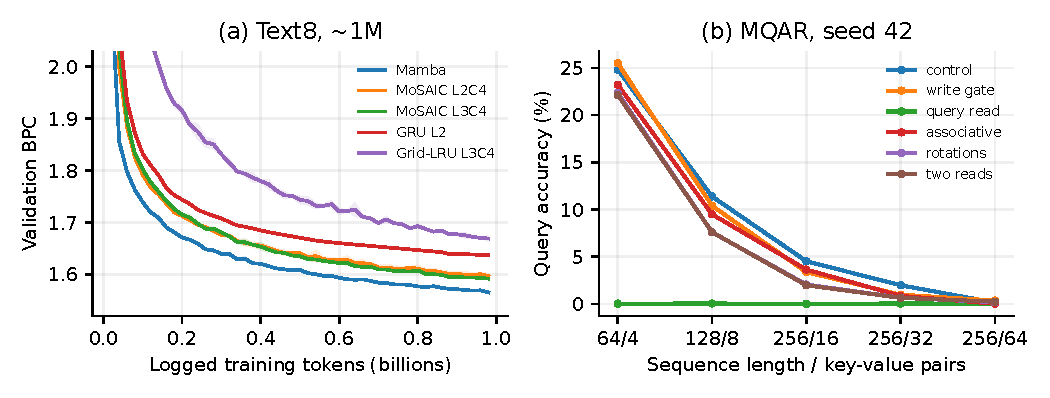
\includegraphics[width=0.92\textwidth]{fig_aistats_mid_memory.pdf}
\caption{Additional evidence. (a) New text8 means and sample-SD bands across launches within each configuration ($n=2$ for Mamba, $n=3$ for the other plotted groups). (b) MQAR per-bin validation query accuracy for the six single-seed LRU pilots. The text8 improvement from two reads does not imply reliable associative retrieval.}
\label{fig:midmemory}
\end{figure}

\section{Uncertainty and Evidence Selection}\label{app:uncertainty}

Means and sample standard deviations are calculated across replicate-level summaries, using final validation BPC for text8 and the final-five-measurement mean for SDQ. Standard-deviation bands in the figures describe between-launch variability and are not confidence intervals. With only two or three launches, neither normality nor a reliable population effect can be established. Historical seed independence and pairing cannot be verified from the retained records. New main runs have recorded seeds; the reported aggregate does not perform a paired significance test. Validation tuning, architecture selection, and multiple comparisons are not accounted for by the sample SD.

The historical cohort is fixed by the original retained run inventory; new main groups use the recorded-seed baseline inventory and frozen quality curves available for this revision. Full-budget results use final evaluations rather than training peaks. All historical shapes, new full-budget baseline groups, and the five LRU mechanism variants are reported. Pilots are explicitly separate from full-budget conclusions. Model/variant selection uses validation rather than test values. A tracker entry without a quality curve, or a metadata flag indicating that it is no longer running, is not treated as a completed quality experiment. In particular, short addressable-slot checks have no full-budget comparative evidence and are not included as recall results.

\section{LRU Extensions and Sparse Communication}\label{app:lru}

\paragraph{Static Grid-LRU.}
The simplified baseline uses independent complex diagonal recurrences with residual public outputs. In schematic form, its private state obeys $\mathbf{s}_t=\boldsymbol{\lambda}\odot\mathbf{s}_{t-1}+\mathbf{B}\mathbf{x}_t$, where real and imaginary coordinates are packed in real tensors. Trainable pole radii are below one; initial e-folding horizons are sampled log-uniformly between 1 and 1,000 recurrent steps. The public output combines a projection of complex state with a direct residual input. Inter-column mixing is a learned row-softmax table independent of the current query, without the GRU model's query/key/value projections, identities, stochastic routing, or auxiliary objectives. Bottom-layer feedback is parameter-free RMS-normalized. Only the top-layer column-0 public output reaches the prediction head. Stable poles constrain the isolated recurrence; they do not bound the coupled grid's nonlinear feedback or guarantee stable training.

\paragraph{Five mechanism pilots.}
These use an L2C4H180 dynamic-hub control with star connectivity, an eight-dimensional query from the hub, zero-initialized query projection, normalized feedback, and no auxiliary loss. Peripheral routes remain query independent; the hub's source weights depend on its previous public output. Every variant keeps the single-column prediction bottleneck. They therefore have a different control from the dense static Grid-LRU in Table~\ref{tab:mid}.

\begin{itemize}
\item \emph{Write gate}: a scalar sigmoid per peripheral column interpolates between its previous private state and the full candidate update, preserving real and imaginary memory when closed; the hub always updates. All projections still execute.
\item \emph{Query-conditioned read}: each peripheral private state is compressed to rank 16, multiplied by a hub-dependent gate, and projected back to the message width only for the hub's read. This changes read contents in addition to source weights.
\item \emph{Associative column}: column 3 is replaced by a $16\times32$ matrix with normalized key $\mathbf{k}$, bounded value $\mathbf{v}$, and sigmoid write rate $\eta$. Its delta update is $\mathbf{M}'=\mathbf{M}+\eta\mathbf{k}(\mathbf{v}-\mathbf{M}^{\mathsf T}\mathbf{k})^{\mathsf T}$. A normalized hub query reads the matrix. This replacement changes both parameter count (about 0.830M versus 1.055M in text8) and state allocation, so it is not a matched-capacity control.
\item \emph{Rotations}: sequential Givens rotations exchange hub/peripheral real and imaginary coordinates before the recurrence, with four groups of angles initialized to zero. Norm preservation of this exchange alone does not establish grid stability.
\item \emph{Two reads}: after an ordinary all-column candidate pass, the hub reads freshly computed peripheral outputs and recomputes its candidate from the original previous hub state using shared weights. Peripherals write once. At four columns this adds approximately 25\% cell-projection arithmetic, plus routing; it is not a measured wall-time estimate.
\end{itemize}

% Generated offline by inference/aistats_revision_evidence.py.
\begin{table}[t]
\centering
\caption{Five LRU mechanisms and their own dynamic-hub control on Text8, seed 42, at 980,037,632 tokens. Late $\Delta$ averages paired differences at the common 800.03--980.04M logs. Reset-1024 evaluates the same validation data with state reset every 1,024 valid tokens; reset penalty is its BPC minus continuous BPC. Core widths are L2C4H180; added projections or replacement of an LRU by matrix memory change parameter/state counts. This is a single-seed exploratory comparison.}
\label{tab:lruvariants}
\begin{tabular}{lrrrrr}
\toprule
Variant & BPC $\downarrow$ & $\Delta$ & Late $\Delta$ & Reset-1024 & Reset penalty \\
\midrule
control & 1.6687 & $+0.0000$ & $+0.0000$ & 1.6803 & $+0.0116$ \\
write gate & 1.6675 & $-0.0012$ & $-0.0014$ & 1.6799 & $+0.0124$ \\
query read & 1.6872 & $+0.0185$ & $+0.0184$ & 1.7009 & $+0.0136$ \\
associative & 1.6938 & $+0.0251$ & $+0.0224$ & 1.7121 & $+0.0183$ \\
rotations & 1.6663 & $-0.0024$ & $-0.0003$ & 1.6787 & $+0.0123$ \\
two reads & 1.6530 & $-0.0157$ & $-0.0168$ & 1.6641 & $+0.0111$ \\
\bottomrule
\end{tabular}
\end{table}


Two reads improves text8 from 1.6673 to 1.6488 BPC; the paired late-window difference is also negative. Write gates and rotations change BPC much less, and query-conditioned/matrix reads worsen it. These are one-seed outcomes, not evidence of a universal memory improvement. The variants also differ in parameter counts, state allocation, or update computation, as specified above.

\paragraph{Periodic-reset diagnostic.}
The retained logs also evaluate the same validation data with each stream's state reset every 1,024 valid tokens, independently of BPTT length. Table~\ref{tab:lruvariants} reports this diagnostic at the same checkpoint. Two reads gives 1.6607 BPC versus 1.6794 for its dynamic-hub control, retaining a 0.0187-BPC advantage. The reset increases BPC by 0.0119 and 0.0120, respectively. This single-seed result shows that the gain persists under periodic resets; it does not establish superior retrieval beyond 1,024 tokens or identify the gain as a longer memory horizon. Late-window averages likewise summarize correlated checkpoints rather than independent repeats.

\paragraph{Sparse LRU pilots.}
The separate suite varies learned mixing initialization/connectivity: self-heavy mixing increases the initial diagonal preference; star routes peripherals through the hub; star-ring adds neighboring links; clockwork updates peripherals on scheduled slower clocks; block factorizes cell projections into smaller channel groups; entmax sparsifies routing probabilities; dynamic hub adds a query-conditioned hub read. All retain column-0 readout. Table~\ref{tab:sparselru} reports validation BPC and differences from the dense control with a 1B-token training budget.

% Generated offline by inference/aistats_revision_evidence.py.
\begin{table}[t]
\centering
\caption{Sparse LRU pilots on Text8, seed 42, with a 1B-token training budget. $\Delta$ is BPC difference from the dense control. Block has a 0.531M core versus approximately 1.05M for its dense control.}
\label{tab:sparselru}
\begin{tabular}{lrr}
\toprule
Variant & BPC $\downarrow$ & $\Delta$ \\
\midrule
self heavy & 1.6680 & $-0.0082$ \\
star & 1.6816 & $+0.0055$ \\
star ring & 1.6828 & $+0.0067$ \\
clockwork & 1.7084 & $+0.0323$ \\
block & 1.7638 & $+0.0877$ \\
entmax & 1.6861 & $+0.0099$ \\
dynamic hub & 1.6659 & $-0.0102$ \\
\bottomrule
\end{tabular}
\end{table}


Self-heavy and dynamic-hub pilots show small paired gains, while block and clockwork lose quality in the tested settings. The block core has about half the dense core's parameters. Sparse attention support alone need not avoid dense projections or recurrent updates; none of these quality logs is a controlled throughput measurement.

\section{BPTT-Length Pilots}\label{app:rollout}

Table~\ref{tab:rollout} compares ordinary GRU, plain LRU, MoSAIC-GRU, and static Grid-LRU at BPTT lengths 64 and 512 across eight launches. Each uses seed 42, the new text8 split, a target of 67,108,864 tokens, no test-based selection, and the same 524,288-token validation cap with 512 evaluation streams. Training streams change from 512 to 64 to keep the token batch at 32,768 and the planned update count equal. The new text8 reset warmup ends near 49.152M tokens, so these pilots primarily describe early training, not convergence at long context.

% Generated offline by inference/aistats_revision_evidence.py.
\begin{table}[t]
\centering
\caption{Rollout pilots at 50,331,648 tokens, seed 42; BPC with the same capped validation. Length 64 uses 512 training streams, length 512 uses 64: both have 32,768 tokens/update. Longer BPTT changes the number of independent streams and does not isolate context length alone.}
\label{tab:rollout}
\begin{tabular}{lrrr}
\toprule
Model & Rollout 64 & Rollout 512 & $\Delta$ \\
\midrule
GRU & 1.9826 & 2.0034 & $+0.0208$ \\
Grid-GRU & 1.9260 & 1.9464 & $+0.0204$ \\
Grid-LRU & 2.4867 & 2.4870 & $+0.0004$ \\
LRU & 2.1575 & 2.1552 & $-0.0022$ \\
\bottomrule
\end{tabular}
\end{table}


GRU and MoSAIC-GRU are about 0.02 BPC worse at length 512; plain LRU changes by $-0.0022$ and Grid-LRU by $+0.0004$. This setting does not demonstrate a benefit from longer gradient propagation. A larger rollout also changes the number of independent trajectories per update and their resets; it cannot alone establish a memory-horizon effect.

\section{Multi-Query Associative Recall Pilots}\label{app:mqar}

The generator follows the single-pass MQAR protocol of Zoology \citep{arora2023zoology}. Vocabulary size is 8,192. Unique keys come from the lower vocabulary half and values from the upper half. A prefix stores alternating keys/values; each key is queried once at a distinct suffix position, with power-law position weighting exponent $0.01-1$. Other positions contain random vocabulary tokens. Only designated queries have supervised targets, at the position of the query key; filler coincidences are not scored. Training, validation, and test sample generators have separate fixed seeds (100/200/300); model/order seed is 42. Sequence state resets for each example, and BPTT spans the full sequence, so there is no truncation between stores and queries.

Training has 100,000 sequences at length/pairs 64/4 and 20,000 at each of 128/8, 256/16, 256/32, and 256/64. Validation has 1,000 independent sequences per training bin. The six pilots override the configured epoch count to eight, use Adam at $10^{-3}$, batch size 32, norm clipping at 1, and query-normalized cross-entropy. At H180, the vocabulary adapters bring full model size to approximately 4M parameters; the core remains near the text8 mid scale, with the mechanism-specific differences noted above. This is not the same full-parameter budget as the text8 tables. We report validation retrieval accuracy and cross-entropy; no test values are used for this comparison.

% Generated offline by inference/aistats_revision_evidence.py.
\begin{table}[t]
\centering
\caption{MQAR pilots at 173,598,720 logged training tokens, seed 42: query-weighted validation accuracy (\%) and cross-entropy (nats), followed by bin accuracies (\%). All sequence-level exact-match accuracies are zero. Each bin contains 1,000 sequences; no strong-baseline or repeated-seed comparison is available.}
\label{tab:mqar}
\begin{tabular}{lrrrrrrr}
\toprule
Variant & Overall & CE & 64/4 & 128/8 & 256/16 & 256/32 & 256/64 \\
\midrule
control & 2.700 & 7.838 & 24.825 & 11.388 & 4.519 & 1.969 & 0.142 \\
write gate & 2.357 & 7.412 & 25.500 & 10.400 & 3.363 & 0.969 & 0.348 \\
query read & 0.023 & 8.322 & 0.025 & 0.037 & 0.006 & 0.041 & 0.017 \\
associative & 2.059 & 8.506 & 23.225 & 9.488 & 3.631 & 0.847 & 0.020 \\
rotations & 1.738 & 7.678 & 22.350 & 7.587 & 2.044 & 0.653 & 0.184 \\
two reads & 1.743 & 7.721 & 22.150 & 7.600 & 1.975 & 0.637 & 0.230 \\
\bottomrule
\end{tabular}
\end{table}


The overall accuracy weights each bin by its number of queries: with equal validation sequence counts, the five weights are $4/124$, $8/124$, $16/124$, $32/124$, and $64/124$. Consequently the 64-pair bin contributes over half the aggregate, whereas the 4-pair bin dominates the training sequence count. For the control, the macro-average bin accuracy is 8.568\%; reweighting validation by training sequence proportions gives about 15.79\%, versus the logged training EMA near 21.12\%. Neither is the reported query-weighted validation accuracy of 2.70\%. This imbalance prevents interpreting their raw ratio as a generalization-gap estimate. Per-bin recall remains poor, including on training-range lengths.

Table~\ref{tab:mqar} shows the per-bin retrieval results. Guessing uniformly over valid values gives $1/4096\approx0.0244\%$ accuracy; the query-read pilot is near this level overall. Its later loss reduction does not imply restored recall. Several runs log extremely large pre-clipping gradient-norm EMAs and some skipped updates; clipping and poles below one did not eliminate all numerical problems in these coupled recurrent models. These diagnostics are smoothed logger values, not exact per-update counts. Rotations avoids the large spikes in this cohort but has low retrieval accuracy. There are no completed repeated-seed GRU/Mamba/Transformer MQAR comparisons, so the pilot characterizes these LRU variants rather than ranking model families.

\section{POPGym Reinforcement-Learning Pilots}\label{app:rl}

We use POPGym \citep{morad2023popgym} environments through the project's RL runner: RepeatPreviousHard requires recalling a delayed past symbol, and AutoencodeEasy requires reconstructing an earlier observed sequence. This is a POPGym pilot, not evaluation on the separate MIKASA benchmark. Ten launches compare six models on RepeatPreviousHard (GRU, plain LRU, MoSAIC-GRU, static Grid-LRU, dynamic hub, two reads) and four on AutoencodeEasy (GRU, plain LRU, dynamic hub, two reads). Models have approximately 1M parameters and use seed 42; Grid readout remains restricted to column 0.

The common PPO setup has 32 environments, rollout length 128, 4,096 vector slots/update, two optimization epochs, $\gamma=0.995$, GAE $\lambda=0.99$, clipping ratio 0.1, value weight 0.5, entropy weight 0.005, gradient clipping at 0.5, and target KL 0.02. The learning rate warms from $10^{-6}$ to $2\times10^{-4}$ over 16 events spaced four updates apart, then moves 1\% toward $10^{-4}$ every 100 updates. The wrapper supplies previous action/reward identically to all models, normalizes readout features, and initializes policy-head gain to 0.01. Recurrent state is refreshed between optimization epochs; reset-only slots are masked. Budget 8,388,608 counts vector slots, not necessarily valid transitions. No communication auxiliary losses or recurrent logit noise are used.

Each evaluation uses a freshly created environment with seed 50000, stochastic actions, 32 completed episodes, and 16 evaluation environments. We average four late evaluations from each training trajectory; they do not supply four independent training replicates. Evaluation uses a fixed seed across checkpoints and may repeatedly sample the same environment instances.

% Generated offline by inference/aistats_revision_evidence.py.
\begin{table}[t]
\centering
\caption{POPGym pilots, seed 42: mean return over four late evaluations. Each evaluation uses 32 stochastic-policy episodes with fresh environment seed 50000. Evaluations share one training trajectory; their mean is not a seed-level uncertainty estimate.}
\label{tab:rl}
\begin{tabular}{llr}
\toprule
Environment & Model & Late return $\uparrow$ \\
\midrule
RepeatPreviousHard & GRU & -0.5161 \\
RepeatPreviousHard & LRU & -0.3809 \\
RepeatPreviousHard & Grid-GRU & -0.4942 \\
RepeatPreviousHard & Grid-LRU & -0.4973 \\
RepeatPreviousHard & dynamic-hub & -0.4963 \\
RepeatPreviousHard & two-reads & -0.4927 \\
AutoencodeEasy & GRU & -0.4964 \\
AutoencodeEasy & LRU & -0.4663 \\
AutoencodeEasy & dynamic-hub & -0.5072 \\
AutoencodeEasy & two-reads & -0.5111 \\
\bottomrule
\end{tabular}
\end{table}


Table~\ref{tab:rl} reports the late evaluation returns. Random guessing has expected return $-0.5$ and perfect prediction $+1$ in these settings. Plain LRU's RepeatPreviousHard mean $-0.3809$ is a modest departure from chance; it is not task mastery or proof of a particular memory strategy. Grid variants remain near chance on both probes. The ten runs have no logged skipped updates, but this does not establish convergence or robust stability. Some Grid-LRU raw states are much larger than those of plain LRU despite bounded poles and normalized feedback. These single-seed pilots require replication before drawing conclusions about RL performance.

\clearpage
% Generated offline by inference/aistats_resource_accounting.py.
\section{Historical Resource Accounting}\label{app:resources}

Resource logs were recovered for the 65 historical launches in the main and reduced-token quality summaries. The tables below restrict resource accounting to the 48 launches whose device logs identify NVIDIA H100 80GB HBM3; the other 17 launches used different GPU types and are excluded from these resource tables. Historical quality summaries retain the complete original cohort, including those launches. Thus hardware-restricted resource counts differ from quality-table counts. No device labels or measurements have been reassigned or converted to H100 equivalents.

For a run with processed-token counter $s_i$ and interval rate $f_i=\texttt{perf/fps}_i$, we reconstruct $T_{\mathrm{loop}}=\sum_i(s_i-s_{i-1})/f_i$, with $s_0=0$, over the training budget. The effective rate is processed tokens divided by $T_{\mathrm{loop}}$. This includes compilation, training, validation, inspection, logging overhead, and any workload contention. These are log-derived elapsed-time proxies rather than dedicated throughput benchmarks or exclusive GPU-hours.

Update counts are $\lfloor s_{\mathrm{last}}/(n_{\mathrm{envs}}\,\ell_{\mathrm{TBPTT}})\rfloor$, counting reached update boundaries; a nonfinite-gradient skip need not perform an optimizer step. Tracker duration and the fps integral disagree in two launches in the complete historical inventory, so metadata duration is not used as the cost estimator. Tables report means $\pm$ sample standard deviations per launch; single-launch rows have no uncertainty estimate. H100 hardware labels do not control concurrent workloads or implementation differences. The new reported experiments also identify H100 80GB HBM3 in their device logs.

\begin{table}[H]
\centering
\caption{SDQ: Main cohort resources, H100 subset only. Training budget: 1B tokens.}
\begin{tabular}{lrrrr}
\toprule
Model & $n$ & Updates (k) & Loop time (h) & Rate (k tokens/s) \\
\midrule
MoSAIC-L1C8 & 3 & $61.03\pm0.00$ & $1.126\pm0.095$ & $248.0\pm22.1$ \\
MoSAIC-L2C16 & 3 & $61.03\pm0.00$ & $1.639\pm0.144$ & $170.4\pm15.7$ \\
MoSAIC-L2C4 & 1 & $61.03$ & $1.327$ & $209.3$ \\
MoSAIC-L2C8 & 3 & $61.03\pm0.00$ & $1.554\pm0.138$ & $179.7\pm16.8$ \\
MoSAIC-L3C4 & 3 & $61.03\pm0.00$ & $1.946\pm0.311$ & $145.4\pm25.1$ \\
GRU-L2 & 1 & $61.03$ & $0.984$ & $282.2$ \\
\bottomrule
\end{tabular}
\end{table}

\begin{table}[H]
\centering
\caption{SDQ: Reduced-token context resources, H100 subset only. Reduced-token rows have different batch and update geometries.}
\begin{tabular}{lrrrrr}
\toprule
Model & $n$ & Tokens (M) & Updates (k) & Loop time (h) & Rate (k tokens/s) \\
\midrule
DeltaNet & 2 & $250.0\pm0.0$ & $61.03\pm0.00$ & $3.261\pm0.042$ & $21.3\pm0.3$ \\
HGRN2 & 2 & $125.0\pm0.0$ & $61.03\pm0.00$ & $2.305\pm0.017$ & $15.1\pm0.1$ \\
mLSTM & 2 & $250.0\pm0.0$ & $61.03\pm0.00$ & $3.065\pm0.026$ & $22.7\pm0.2$ \\
\bottomrule
\end{tabular}
\end{table}

\clearpage
\begin{table}[H]
\centering
\caption{text8: Main cohort resources, H100 subset only. Training budget: 1B tokens.}
\begin{tabular}{lrrrr}
\toprule
Model & $n$ & Updates (k) & Loop time (h) & Rate (k tokens/s) \\
\midrule
MoSAIC-L1C8 & 3 & $30.52\pm0.00$ & $1.213\pm0.097$ & $229.9\pm17.6$ \\
MoSAIC-L2C16 & 2 & $30.52\pm0.00$ & $1.825\pm0.123$ & $152.6\pm10.3$ \\
MoSAIC-L2C4 & 2 & $30.52\pm0.00$ & $1.627\pm0.236$ & $172.5\pm25.1$ \\
MoSAIC-L2C8 & 3 & $30.52\pm0.00$ & $1.633\pm0.146$ & $171.0\pm14.7$ \\
MoSAIC-L3C4 & 3 & $30.52\pm0.00$ & $2.264\pm0.033$ & $122.7\pm1.8$ \\
GRU-L1 & 2 & $30.52\pm0.00$ & $0.925\pm0.103$ & $302.1\pm33.6$ \\
GRU-L2 & 2 & $30.52\pm0.00$ & $1.097\pm0.016$ & $253.1\pm3.6$ \\
GRU-L3 & 2 & $30.52\pm0.00$ & $1.240\pm0.015$ & $223.9\pm2.6$ \\
Transformer-256 & 1 & $30.52$ & $0.571$ & $486.1$ \\
Transformer-64 & 2 & $30.52\pm0.00$ & $0.365\pm0.003$ & $761.9\pm6.4$ \\
\bottomrule
\end{tabular}
\end{table}

\begin{table}[H]
\centering
\caption{text8: Reduced-token context resources, H100 subset only. Reduced-token rows have different batch and update geometries.}
\begin{tabular}{lrrrrr}
\toprule
Model & $n$ & Tokens (M) & Updates (k) & Loop time (h) & Rate (k tokens/s) \\
\midrule
DeltaNet & 2 & $200.0\pm0.0$ & $48.83\pm0.00$ & $3.403\pm0.011$ & $16.3\pm0.1$ \\
HGRN2 & 2 & $100.0\pm0.0$ & $48.83\pm0.00$ & $2.431\pm0.006$ & $11.4\pm0.0$ \\
mLSTM & 2 & $200.0\pm0.0$ & $48.83\pm0.00$ & $3.248\pm0.027$ & $17.1\pm0.1$ \\
\bottomrule
\end{tabular}
\end{table}


\end{document}
